\documentclass[table]{beamer}
%[]中可以使用draft、handout、screen、transparency、trancompress、compress等参数

%指定beamer的模式与主题
\mode<presentation>
{
  \usetheme{Madrid}
%\usetheme{Boadilla}
%\usecolortheme{default}
%\usecolortheme{orchid}
%\usecolortheme{whale}
%\usefonttheme{professionalfonts}
}

%\usetheme{Madrid}
%这里还可以选择别的主题:Bergen, Boadilla, Madrid, AnnArbor, CambridgeUS, Pittsburgh, Rochester, Warsaw, ...
%有导航栏的Antibes, JuanLesPins, Montpellier, ...
%有内容的Berkeley, PaloAlto, Goettingen, Marburg, Hannover, ...
%有最小导航栏的Berlin, Ilmenau, Dresden, Darmstadt, Frankfurt, Singapore, Szeged, ...
%有章和节表单的Copenhagen, Luebeck, Malmoe, Warsaw, ...

%\usecolortheme{default}
%设置内部颜色主题(这些主题一般改变block里的颜色);这个主题一般选择动物来命名
%这里还可以选择别的颜色主题,如默认的和有特别目的的颜色主题default,structure,sidebartab,全颜色主题albatross,beetle,crane,dove,fly,seagull,wolverine,beaver

%\usecolortheme{orchid}
%设置外部颜色主题(这些主题一般改变title里的颜色);这个主题一般选择植物来命名
%这里还可以选择别的颜色主题,如默认的和有特别目的的颜色主题lily,orchid,rose

%\usecolortheme{whale}
%设置字体主题;这个主题一般选择海洋动物来命名
%这里还可以选择别的颜色主题,如默认的和有特别目的的颜色主题whale,seahorse,dolphin

%\usefonttheme{professionalfonts}
%类似的还可以定义structurebold,structuresmallcapsserif,professionalfonts


% 控制 beamer 的风格,可以根据自己的爱好修改
%\usepackage{beamerthemesplit} %使用 split 风格
%\usepackage{beamerthemeshadow} %使用 shadow 风格
%\usepackage[width=2cm,dark,tab]{beamerthemesidebar}

%插入音标
\usepackage{tipa}
\AtBeginDocument{
  \renewcommand\textipa{\fontencoding{T3}\selectfont}
}
\AtBeginDocument{
  \renewcommand\textipa[2][r]{{\fontfamily{cm#1}\tipaencoding #2}}
}
\renewenvironment{IPA}[1][r]
 {\fontfamily{cm#1}\tipaencoding}
 {}

% 设定英文字体
%\usepackage{fontspec}
\usepackage[no-math]{fontspec}
\setmainfont{Times New Roman}
\setsansfont{Arial}
\setmonofont{Courier New}

% 设定中文字体
\usepackage[BoldFont,SlantFont,CJKchecksingle,CJKnumber]{xeCJK}
%\setCJKmainfont[BoldFont={Adobe Heiti Std},ItalicFont={Adobe Kaiti Std}]{Adobe Song Std}
\setCJKmainfont[BoldFont={Adobe Heiti Std},ItalicFont={Adobe Kaiti Std}]{WenQuanYi Micro Hei}
\setCJKsansfont{Adobe Heiti Std}
\setCJKmonofont{Adobe Fangsong Std}
\punctstyle{hangmobanjiao}

\defaultfontfeatures{Mapping=tex-text}
\usepackage{xunicode}
\usepackage{xltxtra}

\XeTeXlinebreaklocale "zh"
\XeTeXlinebreakskip = 0pt plus 1pt minus 0.1pt

\usepackage{setspace}
\usepackage{colortbl,xcolor}
\usepackage{hyperref}
%\hypersetup{xetex,bookmarksnumbered=true,bookmarksopen=true,pdfborder=1,breaklinks,colorlinks,linkcolor=blue,filecolor=black,urlcolor=cyan,citecolor=green}
\hypersetup{xetex,bookmarksnumbered=true,bookmarksopen=true,pdfborder=1,breaklinks,colorlinks,linkcolor=cyan,filecolor=black,urlcolor=blue,citecolor=green}

% 插入图片
\usepackage{graphicx}
\graphicspath{{figures/}}
% 图文混排
\usepackage{picins}
\usepackage{floatflt}

% 可能用到的包
\usepackage{amsmath,amssymb}
%插入多媒体
%\usepackage{media9}
%\usepackage{movie15}
\usepackage{multimedia}
\usepackage{multicol}
\usepackage{multirow}

% 定义一些自选的模板,包括背景、图标、导航条和页脚等,修改要慎重
% 设置背景渐变由10%的红变成10%的结构颜色
%\beamertemplateshadingbackground{red!10}{structure!10}
%\beamertemplatesolidbackgroundcolor{white!90!blue}
% 使所有隐藏的文本完全透明、动态,而且动态的范围很小
\beamertemplatetransparentcovereddynamic
% 使itemize环境中变成小球,这是一种视觉效果
\beamertemplateballitem
% 为所有已编号的部分设置一个章节目录,并且编号显示成小球
\beamertemplatenumberedballsectiontoc
% 将每一页的要素的要素名设成加粗字体
\beamertemplateboldpartpage

% item逐步显示时,使已经出现的item、正在显示的item、将要出现的item呈现不同颜色
\def\hilite<#1>{
 \temporal<#1>{\color{gray}}{\color{blue}}
    {\color{blue!25}}
}

\renewcommand{\today}{\number\year 年 \number\month 月 \number\day 日}

%五角星
\usepackage{MnSymbol}

%去除图表标题中的figure等
\usepackage{caption}
\captionsetup{labelformat=empty,labelsep=none}

\usepackage{tabu}
\usepackage{multirow}
%表格自动换行
\usepackage{tabularx} 

% 千分号
%\usepackage{textcomp}

%罗马数字
\makeatletter
\newcommand{\rmnum}[1]{\romannumeral #1}
\newcommand{\Rmnum}[1]{\expandafter\@slowromancap\romannumeral #1@}
\makeatother

%分栏
\usepackage{multicol}

%\usepackage{enumitem}
%\usepackage{enumerate}

%键盘
\usepackage{keystroke}

%插入源代码
\usepackage{listings}
\lstset{
  language=bash,                  % 程序语言名称:TeX, Perl, R, sh, bash, Awk
  basicstyle=\normalsize\tt,      %\tt指monospace字体族,程序源代码使用此族字体表示更加美观
  numbers=left,                   % 行号位置(左侧)
  numberstyle=\small,             % 行号字体的字号
  stepnumber=1,                   % 行号的显示步长
  numbersep=5pt,                  % 行号与代码间距
  backgroundcolor=\color{white},  % 背景色;需要 \usepackage{color}
  showspaces=false,               % 不显示空格
  showstringspaces=false,         % 不显示代码字符串中的空格标记
  showtabs=false,                 % 不显示 TAB
  tabsize=4, 
  frame=shadowbox,                % 把代码用带有阴影的框圈起来
  captionpos=b,                   % 标题位置
  breaklines=true,                % 对过长的代码自动断行
  breakatwhitespace=false,        % 断行只在空格处
  extendedchars=false,            % 解决代码跨页时,章节标题,页眉等汉字不显示的问题
  %escapeinside={\%*}{*},         % 跳脱字符,添加注释,暂时离开 listings 
  %escapeinside=``,
  commentstyle=\color{red!50!green!50!blue!50}\tt,  %浅灰色的注释
  rulesepcolor=\color{red!20!green!20!blue!20},     %代码块边框为淡青色
  keywordstyle=\color{blue!70}\bfseries\tt,         %代码关键字的颜色为蓝色,粗体
  identifierstyle=\tt,
  stringstyle=\tt,                % 代码字符串的特殊格式
  keepspaces=true,
  breakindent=1em,
  %breakindent=22pt,
  %breakindent=4em,
  breakautoindent=true,
  flexiblecolumns=true,
  aboveskip=1em,                  %代码块边框
  xleftmargin=2em,
  xrightmargin=2em
}

%\setbeamercolor{alerted text}{fg=magenta}
\setbeamercolor{bgcolor}{fg=yellow,bg=cyan}
%\setbeamercolor{itemize/enumerate body}{fg=green}

\begin{document}

%\includeonlyframes{current}

\logo{
\includegraphics[height=0.08\textwidth]{tijmu.png}}

% 在每个Section前都会加入的Frame
\AtBeginSection[]
{
  \begin{frame}<beamer>
    %\frametitle{Outline}
    \frametitle{教学提纲}
    \setcounter{tocdepth}{3}
    \begin{multicols}{2}
      \tableofcontents[currentsection,currentsubsection]
      %\tableofcontents[currentsection]
    \end{multicols}
  \end{frame}
}
% 在每个Subsection前都会加入的Frame
\AtBeginSubsection[]
{
  \begin{frame}<beamer>
%%\begin{frame}<handout:0>
%% handout:0 表示只在手稿中出现
    \frametitle{教学提纲}
    \setcounter{tocdepth}{3}
    \begin{multicols}{2}
    \tableofcontents[currentsection,currentsubsection]
    \end{multicols}
%% 显示在目录中加亮的当前章节
  \end{frame}
}

% 为当前幻灯片设置背景
%{
%\usebackgroundtemplate{
%\vbox to \paperheight{\vfil\hbox to
%\paperwidth{\hfil
\includegraphics[width=2in]{tijmu_charcoal.png}\hfil}\vfil}
%}
\begin{frame}[plain]
  \begin{center}
    {\Huge Linux系统概论\\}
    \vspace{1cm}
    {\LARGE 天津医科大学\\}
    %\vspace{0.2cm}
    {\LARGE 生物医学工程与技术学院\\}
    \vspace{1cm}
    {\large 2017-2018学年下学期(春)\\ 2016级生信班}
  \end{center}
\end{frame}
%}



%\includeonlyframes{current}

\title[常用Linux命令]{第四章\quad 常用Linux命令}
\author[Yixf]{伊现富(Yi Xianfu)}
\institute[TIJMU]{天津医科大学(TIJMU)\\ 生物医学工程与技术学院}
\date{2019年5月}


\begin{frame}
  \titlepage
\end{frame}

\begin{frame}[plain,label=current]
  \frametitle{教学提纲}
  \setcounter{tocdepth}{3}
  \begin{multicols}{2}
    \tableofcontents
  \end{multicols}
\end{frame}


\section{引言}
\begin{frame}
  \frametitle{引言 | 命令}
  \begin{block}{命令}
    \begin{itemize}
      \item 命令是可执行的程序,使得用户能够要求机器执行某种操作
      \item 有时候是shell的内置功能,如:列出目录的内容
      \item 有时候是单独的程序,如:设置机器运行时的基本参数的一长串脚本
    \end{itemize}
  \end{block}
\end{frame}

\begin{frame}
  \frametitle{引言 | \alert{进入命令行界面}}
  \begin{block}{远程登录}
    \begin{itemize}
      \item ssh \textcolor{gray}{USERNAME@}HOSTNAME
    \end{itemize}
  \end{block}
  \pause
  \begin{block}{本地桌面}
    \begin{itemize}
      \item 开机直接进入:不安装图形界面(只有命令行界面可用)
      \item 虚拟终端(从图形界面完全切换到命令行界面):Ctrl + Alt + F[1-6]/F[2-7]
      \item 终端模拟器(在图形界面中使用命令行):打开Terminal/终端
      \item \textcolor{gray}{从命令行界面切换回图形界面:Ctrl + Alt + F7/F1}
    \end{itemize}
  \end{block}
\end{frame}


\section{命令的剖析}
\begin{frame}
  \frametitle{\alert{命令剖析}}
  \begin{figure}
    \centering
    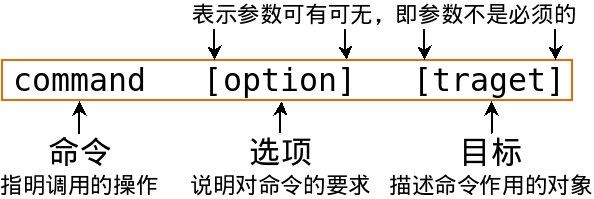
\includegraphics[width=9cm]{c4_command.png}
  \end{figure}
  \pause
  \begin{block}{Linux命令}
    %\begin{itemize}[<+-|alert@+>]
    \begin{itemize}[<+->]
      \item Linux命令 = 命令 + [参数] (command + [argument])
      \item 命令参数 = [选项] + [目标] ([option] + [target])
      \item 分隔符:空格(Space)
    \end{itemize}
  \end{block}
\end{frame}

\begin{frame}
  \frametitle{命令剖析 | 实例}
  \begin{figure}
    \centering
    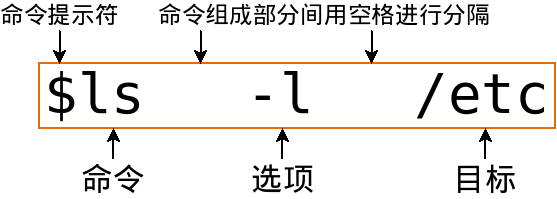
\includegraphics[width=7cm]{c4_command_ls.png}
  \end{figure}
  \pause
  %\begin{itemize}[<+-|alert@+>]
  \begin{itemize}[<+->]
    \item 大多数命令名与该命令所调用的操作在字面上是一样的(ls: list)
    \item 单独执行命令时所发生的一切称为命令的默认行为(ls)
    \item 参数能够影响命令的输出格式以及它的操作(-l /etc)
    \item 目标为命令提供了所要处理的目标位置(/etc)
    \item 有些命令要求多个目标(cp source destination)
    \item 特定的命令通常具有自己独特的选项/开关/标记(-l)
    \item 选项通常(但不一定)位于一个或两个连字符之后(-a = -\!-all)
    \item 多个选项可以独立或是合并添加(-a -l = -al)
  \end{itemize}
\end{frame}


\section{查找命令的相关信息}
\begin{frame}
  \frametitle{命令信息 | 文档来源}
  \begin{enumerate}
    \item The man pages (short for manual pages)
    \item GNU Info
    \item The help command and -\!-help option
    \item Other Documentation Sources
  \end{enumerate}
  \begin{figure}
    \centering
    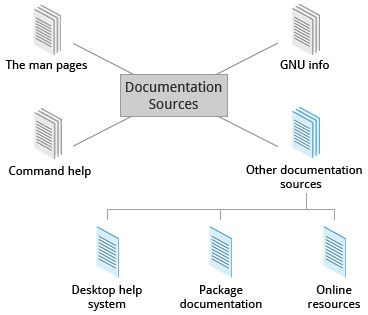
\includegraphics[width=6cm]{c4_help_source.jpg}
  \end{figure}
\end{frame}

\subsection{man}
\begin{frame}[fragile]
  \frametitle{命令信息 | man}
  \begin{block}{man}
    \alert{man COMMAND/CONFIG}:联机帮助页是了解任何特定命令或配置文件的最佳方法(\verb|man passwd| vs. \verb|man 5 passwd|)
  \end{block}
  \begin{figure}
    \centering
    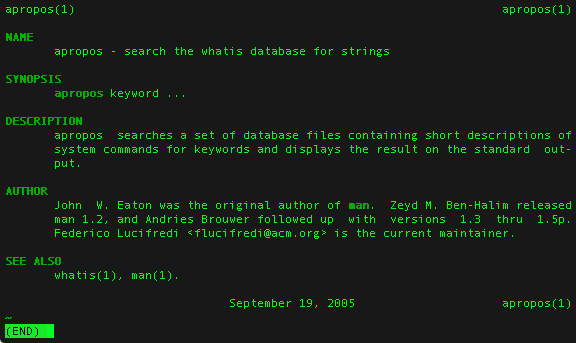
\includegraphics[width=9cm]{c4_man_apropos.png}
  \end{figure}
\end{frame}

\begin{frame}[fragile]
  \frametitle{命令信息 | man | 章节(数字)}
  \begin{table}
    \centering
    \rowcolors[]{1}{blue!20}{blue!10}
    \begin{tabular}{cll}
      \hline
      \rowcolor{blue!50}章节/数字 & 内容/含义 & 补充说明\\
      \hline
      1 & 可执行程序或shell命令 & 可由任何人启动 \\
      2 & 系统调用 & 内核提供的函数\\
      3 & 库调用 & 程序库中的函数\\
      4 & 特殊文件 & 通常位于 /dev\\
      5 & 文件格式和规范 & 如 /etc/passwd\\
      6 & 游戏 & ---\\
      7 & 杂项(包括宏包和规范) & 如man(7), groff(7)\\
      8 & 系统管理命令 & 通常只针对root用户\\
      9 & 内核例程 & 非标准,Linux特有\\
      \hline
    \end{tabular}
  \end{table}
  \pause
  \begin{itemize}
    \item 限定章节:\verb|man 3 printf|
    \item 所有章节:\verb|man -a printf|
  \end{itemize}
\end{frame}

\subsection{info}
\begin{frame}
  \frametitle{命令信息 | info}
  \begin{block}{info}
    info KEYWORD:访问命令的信息帮助页(info page)
  \end{block}
  \begin{figure}
    \centering
    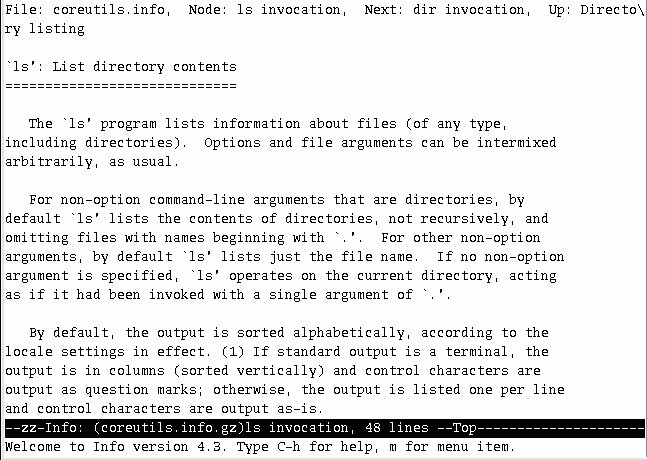
\includegraphics[width=8cm]{c4_info_ls.png}
  \end{figure}
\end{frame}

\subsection{-\!-help/-h}
\begin{frame}[fragile]
  \frametitle{命令信息 | -\!-help}
  \begin{block}{-\!-help}
    \alert{COMMAND -\!-help}:显示命令的帮助信息;\alert{CMD -h}\\
    \verb|help BUILD-IN SHELL CMD|:例如 \verb|help echo|
  \end{block}
  \vspace{-0.2cm}
  \begin{figure}
    \centering
    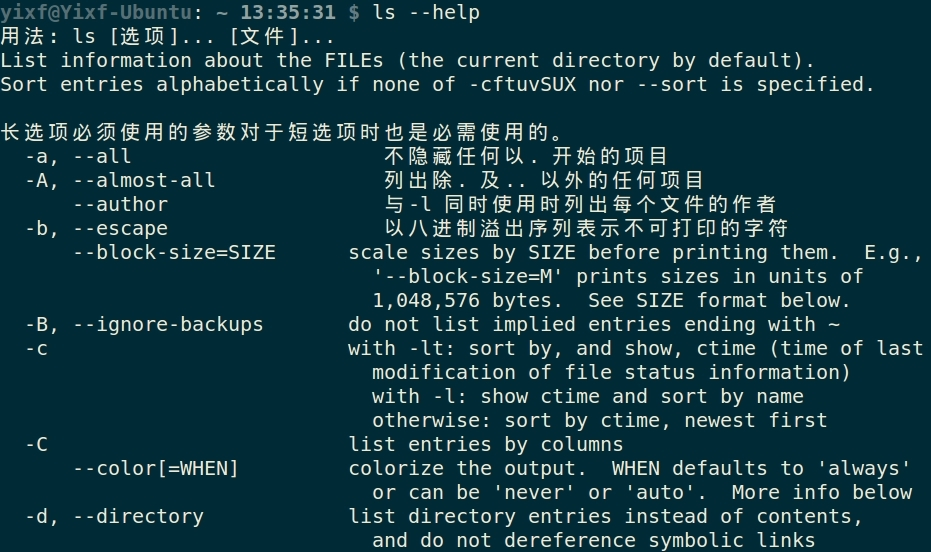
\includegraphics[width=10cm]{c4_ls_help.png}
  \end{figure}
\end{frame}

\subsection{其他命令}
\begin{frame}
  \frametitle{命令信息 | 其他命令}
  \begin{block}{其他命令}
    \begin{itemize}
      \item which COMMAND:查找命令
      \item whereis COMMAND:查找软件包
      \item whatis COMMAND:获得索引的简单说明信息,相当于man -f
      \item apropos KEYWORD:使用关键字来查找相关文件,相当于man -k
      \item makewhatis:建立whatis和apropos搜索使用的数据库
    \end{itemize}
  \end{block}
  \begin{figure}
    \centering
    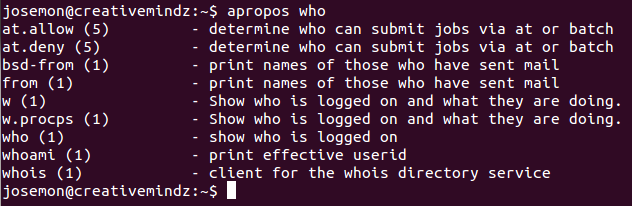
\includegraphics[width=11cm]{c4_apropos_who.png}
  \end{figure}
\end{frame}

\begin{frame}[fragile]
  \frametitle{命令信息 | man vs. info vs. -\!-help}
  \begin{block}{man}
    man可以显示系统手册页中的内容,这些内容大多数都是对命令的解释信息,这些信息是操作系统文档里面的。如果没有文档,是不会显示这些帮助信息的。一般比help出来的要详细。
  \end{block}
  \pause
  \begin{block}{info}
    info是一个基于菜单的超文本系统,由GNU项目开发并由Linux发布。info工具包括一些关于Linux Shell、工具、GNU项目开发程序的说明文档。
  \end{block}
  \pause
  \begin{block}{-\!-help}
-\!-help并不是一个独立的工具,而是一个工具选项,可以用来显示一些工具的信息。这些帮助信息是程序的作者加上去的,也就是说,这些信息是程序内部的。一般比man出来的要简单。
  \end{block}
\end{frame}

\section{命令的修改}
\subsection{元字符}
\begin{frame}
  \frametitle{命令修改 | 元字符}
  \begin{block}{元字符}
    %\begin{itemize}[<+-|alert@+>]
    \begin{itemize}[<+->]
      \item 元字符(metacharacter)并不是命令本身的一部分,但它们是shell的特性,能够让用户创建复杂的操作。
      \item 元字符是正则表达式的一个重要方面。
      \item 最流行的元字符称为通配符(wildcard)。
    \end{itemize}
  \end{block}
  \pause
  \begin{block}{通配符}
    %\begin{itemize}[<+-|alert@+>]
    \begin{itemize}[<+->]
      \item 通配符是专用字符,能够用于同时匹配多个文件,从而增大一次性找到想要的文件名或目标的可能性。
      \item 通配符是一种命令行的路径扩展(path expansion)功能,只作用在argument的path上。
      \item 指定工作目录中的所有word文件(*.doc)
      \item 指定工作目录中的所有以txt或text为后缀的文本文件(*.t[ex]*)
    \end{itemize}
  \end{block}
\end{frame}

\begin{frame}
  \frametitle{命令修改 | 元字符 | \alert{通配符}}
  \begin{figure}
    \centering
    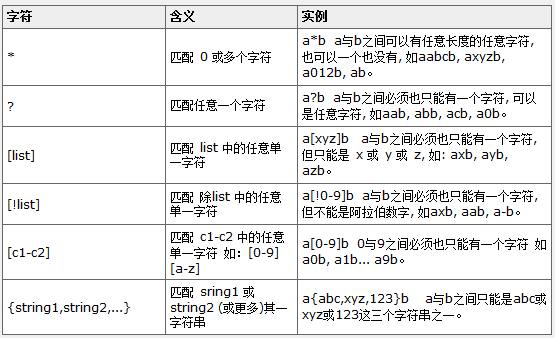
\includegraphics[width=11cm]{c4_metacharacter.png}
  \end{figure}
\end{frame}

\begin{frame}
  \frametitle{命令修改 | 元字符 | 通配符}
  \begin{figure}
    \centering
    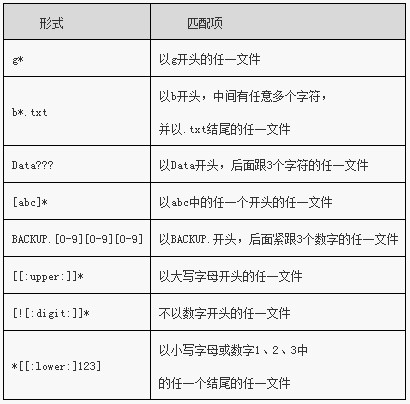
\includegraphics[width=8cm]{c4_metacharacter_example.jpg}
  \end{figure}
\end{frame}

\subsection{转义符}
\begin{frame}[fragile]
  \frametitle{命令修改 | \alert{转义符}}
  \begin{figure}
    \centering
    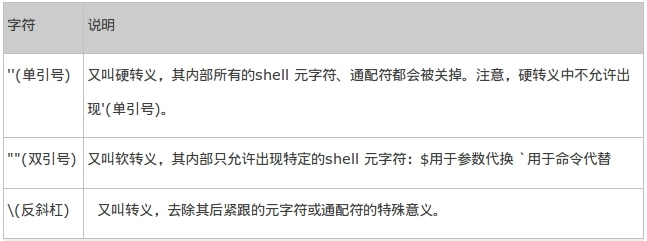
\includegraphics[width=12cm]{c4_shell_01.png}
  \end{figure}
  \pause
  \vspace{-1em}
  \begin{columns}
    \column{0.55\textwidth}
  \begin{block}{转义符使用}
    \begin{itemize}
      \item 使用单引号:\verb|echo '$SHELL'|
      \item 使用双引号:\verb|echo "$SHELL"|
      \item 使用反斜杠:\verb|echo \$SHELL|
    \end{itemize}
  \end{block}
    \column{0.4\textwidth}
    \pause
    \pause
    \begin{block}{输出结果}
      \begin{itemize}
        \item \verb|$SHELL|
        \item \verb|/bin/bash|
        \item \verb|$SHELL|
      \end{itemize}
    \end{block}
  \end{columns}
\end{frame}

\subsection{输入输出重定向}
\begin{frame}
  \frametitle{命令修改 | \alert{输入输出}}
  \begin{table}
    \centering
    \rowcolors[]{1}{blue!20}{blue!10}
    \begin{tabular}{ccccl}
      \hline
      \rowcolor{blue!50}名称 & 说明 & 编号 & 默认 & 作用\\
      \hline
      STDIN(standard input) & 标准输入 & 0 & 键盘 & 接收参数或数据\\
      STDOUT(standard output) & 标准输出 & 1 & 屏幕 & 输出结果\\
      STDERR(standard error) & 标准错误 & 2 & 屏幕 & 输出错误\\
      \hline
    \end{tabular}
  \end{table}
  \begin{figure}
    \centering
    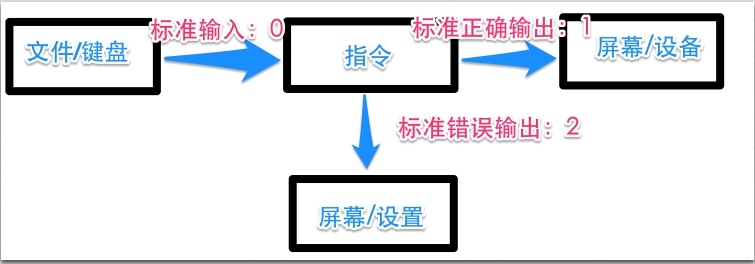
\includegraphics[width=10cm]{c4_io_01.jpg}
  \end{figure}
\end{frame}

\begin{frame}[fragile]
  \frametitle{命令修改 | \alert{重定向}}
  \begin{table}
    \centering
    \rowcolors[]{1}{blue!20}{blue!10}
    \begin{tabular}{cll}
      \hline
      \rowcolor{blue!50}字符 & 说明 & 实例\\
      \hline
      < & 重定向STDIN & \verb|sort < sort.in|\\
      > & 将STDOUT重定向到文件(覆盖) & \verb|ls > ls.out|\\
      \verb|>>| & 将STDOUT重定向到文件(追加) & \verb|date >> date.out|\\
      2> & 将STDERR重定向到文件(覆盖) & \verb|ls no 2> ls.err|\\
      2>\&1 & 将STDERR与STDOUT结合 & \verb|ls no 2>&1 ls.all|\\
      < > & 结合输入输出重定向 & \verb|sort <IN >OUT|\\
      \hline
    \end{tabular}
  \end{table}
\end{frame}

\subsection{管道}
\begin{frame}[fragile]
  \frametitle{命令修改 | \alert{管道}}
  \begin{block}{管道}
    \begin{itemize}
      \item 管道(pipe)是一个操作符,它把输入和输出重定向结合在一起,从而将一个命令的输出立即作为另一个命令的输入。
      \item 管道用垂直线字符(\verb=|=)表示。
      \item \verb=ls -l /etc | less=
    \end{itemize}
  \end{block}
  \begin{figure}
    \centering
    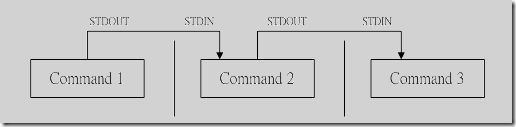
\includegraphics[width=10cm]{c4_pipe.png}
  \end{figure}
\end{frame}

\subsection{命令置换}
\begin{frame}[fragile]
  \frametitle{命令修改 | \alert{命令置换}}
  \begin{block}{命令置换}
    \begin{itemize}
      \item 命令置换也是一种将一个命令的输出作为另一个命令的参数的方法。
      %\item 有三种命令置换的方法:\verb|$()|,\verb|``|,\verb|${}|
      \item 有两种命令置换的方法:
	\begin{itemize}
	  \item 新式写法[推荐]:\verb|$()|
	  \item 旧式写法:\verb|``|
	\end{itemize}
    \end{itemize}
  \end{block}
  \pause
  \begin{block}{实例}
    %\begin{itemize}[<+-|alert@+>]
    \begin{itemize}[<+->]
      \item \verb|ls $(pwd)|
      \item \verb|ls `pwd`|
      %\item \verb|ls ${pwd}|
      \item 等同于 \verb|ls| 或者 \verb|ls .|
    \end{itemize}
  \end{block}
\end{frame}

\section{常用命令汇总}
\subsection{目录操作}
\begin{frame}
  \frametitle{常用命令 | \alert{目录操作}}
  \begin{table}
    \centering
    \rowcolors[]{1}{blue!20}{blue!10}
    \begin{tabular}{ccl}
      \hline
      \rowcolor{blue!50}命令 & 助记 & 说明\\
      \hline
      pwd & Print Work Directory & 显示当前目录\\
      ls & LiSt & 列出目录的内容\\
      cd & Change Directory & 切换目录\\
      mkdir & MaKe DIRectory & 创建目录\\
      rmdir & ReMove DIRectory & 删除空目录\\
      tree & TREE-like & 展示树形的目录结构\\
      du & Disk Usage & 显示目录空间占用情况\\
      \hline
    \end{tabular}
  \end{table}
\end{frame}

\begin{frame}
  \frametitle{常用命令 | 目录操作 | \alert{ls}}
  \begin{table}
    \centering
    \rowcolors[]{1}{blue!20}{blue!10}
    \begin{tabular}{ccl}
      \hline
      \rowcolor{blue!50}选项 & 助记 & 说明\\
      \hline
      -a & All & 列出目录的所有内容,包括隐藏文件\\
      -i & Inode & 列出目录内容,包括inode或磁盘索引号\\
      -l & Long & 用长格式(大小、权限等信息)列出目录的内容\\
      -R & Recursive & 列出目录内容,包括所有的子目录以及它们的内容\\
      -r & Reverse & 排序时反向排序\\
      -S & Size & 依据文件大小(由大到小)列出目录内容\\
      -t & Time & 依据时间标记(上一次的修改时间)列出目录内容\\
      \hline
    \end{tabular}
  \end{table}
\end{frame}

\subsection{文件操作}
\begin{frame}
  \frametitle{常用命令 | \alert{文件操作}}
  \begin{table}
    \centering
    \rowcolors[]{1}{blue!20}{blue!10}
    \begin{tabularx}{\textwidth}{ccX}
      \hline
      \rowcolor{blue!50}命令 & 助记 & 说明\\
      \hline
      file & --- & 识别文件类型(二进制、文本等)\\
      echo & --- &  显示文本、打印信息\\
      cat & conCATenate & 显示一个文件\\
      tac & --- & 逆序显示一个文件\\
      touch & --- & 创建文件或者修改现有文件的属性\\
      cp & CoPy & 复制文件/目录\\
      mv & MoVe & 移动文件/目录或重命名文件/目录\\
      rm & ReMove & 删除文件\\
      ln & LiNk & 创建链接\\
      stat & STATus & 查看文件详细时间参数\\
      \hline
      rsync & Remote SYNChronize & 复制/同步/备份文件\\
      dd & Data Definition & 转换并复制文件/分区/磁盘(Disk Destroyer,Delete Data)\\
      \hline
    \end{tabularx}
  \end{table}
\end{frame}

\begin{frame}
  \frametitle{常用命令 | \alert{文件操作(续)}}
  \begin{table}
    \centering
    \rowcolors[]{1}{blue!20}{blue!10}
    \begin{tabularx}{\textwidth}{ccX}
      \hline
      \rowcolor{blue!50}命令 & 助记 & 说明\\
      \hline
      head & --- & 显示文件的开始部分\\
      tail & --- & 显示文件的结尾部分\\
      more & --- & 从头到尾浏览一个文件(只能向下翻页)\\
      less & --- & \footnotesize{从开头或结尾开始浏览整个文件(可上下翻页)}\\
      wc & Word Count & 计算文件行、字(符)数\\
      sort & --- & 对命令或文件的输出进行排序\\
      uniq & --- & 报告或删除重复的行\\
      cut & --- & 以行为处理对象切割数据字段/列\\
      tee & --- & 将命令的输出发送到多个位置\\
      diff/diff3 & --- & 逐行比较两/三个文本文件,列出其不同之处\\
      patch & --- & 使用diff的结果来完成打补丁的工作\\
      comm & --- & 对两个有序的文件进行比较\\
      cmp & CoMPare & 比较两个文件是否有差异\\
      \hline
    \end{tabularx}
  \end{table}
\end{frame}

\begin{frame}[fragile]
  \frametitle{常用命令 | 文件操作 | echo}
  \begin{figure}
    \centering
    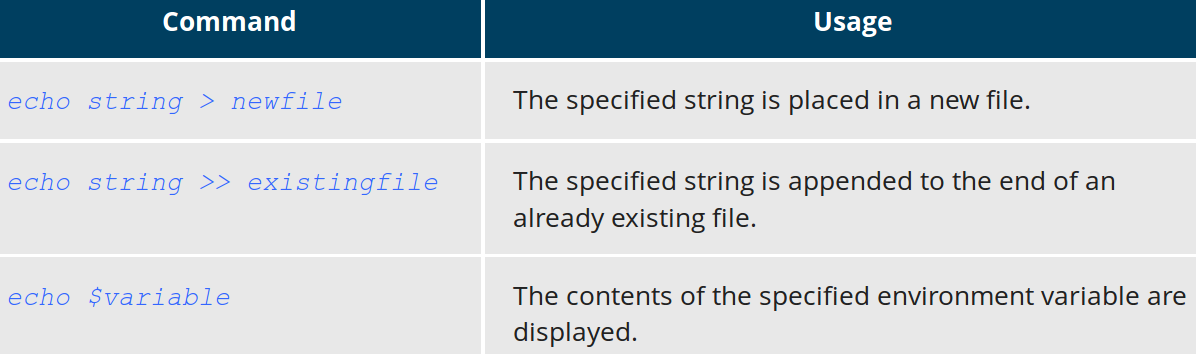
\includegraphics[width=12cm]{c4_echo.png}
  \end{figure}
  \pause
  \begin{block}{\alert{-e}}
    \begin{itemize}
      \item 启用反斜线控制字符(如 \verb|\n|,\verb|\t| 等转义字符)的转换
      \item \verb|echo "line1\tline2"|(输出:\verb|line1\tline2|)
      \item \verb|echo -e "line1\tline2"|(输出:\verb|line1    line2|)
    \end{itemize}
  \end{block}
\end{frame}

\begin{frame}[fragile]
  \frametitle{常用命令 | 文件操作 | cat}
  \begin{table}
    \centering
    \rowcolors[]{1}{blue!20}{blue!10}
    \begin{tabularx}{0.9\textwidth}{ccX}
      \hline
      \rowcolor{blue!50}选项 & 助记 & 说明\\
      \hline
      -e & --- & 等同于 \verb|-vE|\\
      -E & End & 在每一行的结尾显示一个 \verb|$| 字符\\
      -n & Number & 在每一行的开头显示行号\\
      -s & Squeeze & 将连续的空行合并成一个空行\\
      -t & Tabs & 将非打印字符tab显示成 \verb|^I|\\
      -v & --- & 显示所有的非打印字符\\
      \hline
    \end{tabularx}
  \end{table}
  \vspace{-0.5em}
  \pause
  \begin{block}{基本用法}
    \begin{itemize}
      \item 将多个文件的内容依次输出到屏幕上
      \item \verb|cat file1 file2 file3|
    \end{itemize}
  \end{block}
  \vspace{-0.5em}
  \pause
  \begin{block}{\alert{妙用:将多个文件连接成一个更长的新文件}}
    \begin{itemize}
      \item \verb|cat file1 file2 file3 > newfile|
      \item \verb|cat chr{{1..22},X,Y,M}.fa > human_genome.fa|
    \end{itemize}
  \end{block}
\end{frame}

\begin{frame}[fragile]
  \frametitle{常用命令 | 文件操作 | cat}
  \begin{figure}
    \centering
    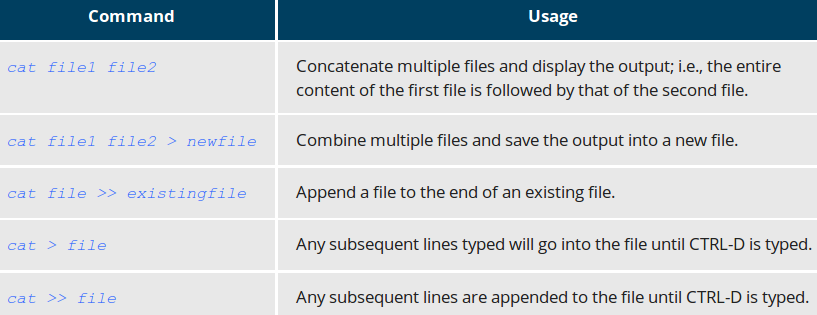
\includegraphics[width=12cm]{c4_cat.png}
  \end{figure}
\end{frame}

\begin{frame}[fragile]
  \frametitle{常用命令 | 文件操作 | \alert{mv}}
  \begin{table}
    \centering
    \rowcolors[]{1}{blue!20}{blue!10}
    \begin{tabularx}{0.9\textwidth}{ccX}
      \hline
      \rowcolor{blue!50}old & new & \verb|mv old new|\\
      \hline
      目录 & 目录 & 移动目录及其中的内容\\
      文件 & 新的文件名 & 重命名文件\\
      文件 & 新的目录 & 移动文件,文件名保持不变\\
      文件 & 新的目录/新的文件名 & 移动文件并进行重命名\\
      \hline
    \end{tabularx}
  \end{table}
\end{frame}

\begin{frame}[fragile]
  \frametitle{常用命令 | 文件操作 | \alert{rm}}
  \begin{table}
    \centering
    \rowcolors[]{1}{blue!20}{blue!10}
    \begin{tabularx}{0.9\textwidth}{ccX}
      \hline
      \rowcolor{blue!50}选项 & 助记 & 说明\\
      \hline
      -f & Force & 使用强制模式,忽略所有警告\\
      -i & Interactive & 使用交互模式,提示用户确认每个删除\\
      -r & Recursive & 使用递归模式,删除所有子目录以及它们包含的文件\\
      \hline
    \end{tabularx}
  \end{table}
\end{frame}

\begin{frame}[fragile]
  \frametitle{常用命令 | 文件操作 | \alert{wc}}
  \begin{table}
    \centering
    \rowcolors[]{1}{blue!20}{blue!10}
    \begin{tabularx}{0.9\textwidth}{ccX}
      \hline
      \rowcolor{blue!50}选项 & 助记 & 说明\\
      \hline
      -c & byte Counts & 显示文件中字符的总数\\
      -l & Line & 显示文件的总行数\\
      -L & Longest/Length & 显示文件中最长一行的长度\\
      -w & Word & 显示文件中单词的总数\\
      \hline
    \end{tabularx}
  \end{table}
\end{frame}

\begin{frame}
  \frametitle{常用命令 | 文件操作 | \alert{sort}}
  \begin{table}
    \centering
    \rowcolors[]{1}{blue!20}{blue!10}
    \begin{tabularx}{0.9\textwidth}{ccX}
      \hline
      \rowcolor{blue!50}选项 & 助记 & 说明\\
      \hline
      -d & Dictionary & 以字典的顺序进行排序,忽略非字符、数字和空格\\
      -f & --- & 排序时忽略大小写\\
      -g & General-number & 按数值排序\\
      -k & Key & 以第几个字段进行排序\\
      -M & Month & 按月份排序\\
      -m & Merge & 合并经过排序的文件\\
      -n & Numeric & 以数值大小进行排序\\
      -R & Random & 随机排序\\
      -r & Reverse & 倒序排序\\
      -t & --- & 指定分隔符\\
      -u & Unique & 排序,只考虑唯一的值\\
      -V & Version & 版本号排序(能正确排序字符数字混杂的情况,如:chr1,chr2,chr10,...)\\
      \hline
    \end{tabularx}
  \end{table}
\end{frame}

\begin{frame}
  \frametitle{常用命令 | 文件操作 | \alert{uniq}}
  \begin{table}
    \centering
    \rowcolors[]{1}{blue!20}{blue!10}
    \begin{tabularx}{0.9\textwidth}{ccX}
      \hline
      \rowcolor{blue!50}选项 & 助记 & 说明\\
      \hline
      -c & Count & 统计每行重复的次数\\
      -d & Dupicate & 只显示重复行\\
      -u & Unique & 只显示没有重复的行\\
      \hline
    \end{tabularx}
  \end{table}
\end{frame}

\begin{frame}
  \frametitle{常用命令 | 文件操作 | \alert{cut}}
  \begin{table}
    \centering
    \rowcolors[]{1}{blue!20}{blue!10}
    \begin{tabularx}{0.9\textwidth}{cclX}
      \hline
      \rowcolor{blue!50}选项 & 助记 & 说明 & 实例\\
      \hline
      -d & Delimiter & 指定分隔符 & -d:\\
      -f & Fields & 表示取第几个字段 & -f1; -f1,5; -f1-5\\
      \hline
    \end{tabularx}
  \end{table}
\end{frame}

\subsection{权限管理}
\begin{frame}
  \frametitle{常用命令 | \alert{权限管理}}
  \begin{table}
    \centering
    \rowcolors[]{1}{blue!20}{blue!10}
    \begin{tabularx}{0.9\textwidth}{ccX}
      \hline
      \rowcolor{blue!50}命令 & 助记 & 说明\\
      \hline
      chown & CHange OWNer & 改变文件或目录的所有者\\
      chgrp & CHange GRouP & 改变文件或目录的所属组\\
      chmod & CHange MODe & 修改权限\\
      useradd & --- & 添加用户帐号\\
      usermod & --- & 修改用户账户的属性\\
      userdel & --- & 删除用户帐号\\
      groupadd & --- & 添加组账户\\
      groupmod & --- & 修改组账户的属性\\
      groupdel & --- & 删除组账户\\
      passwd & PASSWorD & 修改密码\\
      umask & --- & 显示、设置默认的权限方案\\
      \hline
    \end{tabularx}
  \end{table}
\end{frame}

\begin{frame}
  \frametitle{常用命令 | \alert{权限管理}}
  \begin{table}
    \centering
    \rowcolors[]{1}{blue!20}{blue!10}
    \begin{tabularx}{0.9\textwidth}{ccX}
      \hline
      \rowcolor{blue!50}命令 & 助记 & 说明\\
      \hline
      w & Who & 显示登录的用户\\
      who & --- & 显示当前所有登录用户的信息\\
      whoami & --- & 显示当前用户名\\
      who am i & --- & 最初作为什么用户登录\\
      last & --- & 显示用户最近登录信息\\
      finger & --- & 显示用户的相关信息\\
      id & --- & 显示登录的用户以及用户的组的相关信息\\
      groups & --- & 显示用户所属的组\\
      \hline
    \end{tabularx}
  \end{table}
\end{frame}

\subsection{系统导航}
\begin{frame}
  \frametitle{常用命令 | \alert{系统导航}}
  \begin{table}
    \centering
    \rowcolors[]{1}{blue!20}{blue!10}
    \begin{tabularx}{\textwidth}{ccX}
      \hline
      \rowcolor{blue!50}命令 & 助记 & 说明\\
      \hline
      which & --- & \scriptsize{如果文件位于用户的PATH内,则显示文件位置}\\
      whereis & --- & 显示程序名文件的位置\\
      find & --- & 在目录结构中查找文件/目录\\
      locate & --- & 通过名字在数据库中查找文件\\
      updatedb & UPDATE DataBase & 建立整个系统目录文件的数据库\\
      alias & --- & 查看别名信息\\
      df & Disk Free & 显示磁盘空间的使用情况\\
      mount & --- & 挂载文件系统\\
      date & --- & 显示当前日期和时间\\
      cal & CALendar & 显示当月的日历\\
      \hline
      set & --- & 显示/设置shell变量\\
      env & ENVironment & 显示/设置用户变量\\
      export & --- & \footnotesize{显示/设置导出成用户变量的shell变量}\\
      unset & --- & 清除环境变量\\
      \hline
    \end{tabularx}
  \end{table}
\end{frame}

%find will be included in chapter5
%\begin{frame}[fragile]
  %\frametitle{常用命令 | 系统导航 | find}
  %\begin{table}
    %\centering
    %\rowcolors[]{1}{blue!20}{blue!10}
    %\begin{tabularx}{0.9\textwidth}{cX}
      %\hline
      %\rowcolor{blue!50}选项 & 说明\\
      %\hline
      %\verb|--help| & 显示帮助信息\\
      %\verb|--maxdepth n| & 向下搜索到第n层目录\\
      %\verb|--mindepth n| & 至少向下搜索n层子目录\\
      %\verb|--mount| & 防止搜索其他文件系统\\
      %\hline
    %\end{tabularx}
  %\end{table}
%\end{frame}

%\begin{frame}
  %\frametitle{常用命令 | 系统导航 | \alert{find}}
  %\begin{table}
    %\centering
    %\rowcolors[]{1}{blue!20}{blue!10}
    %\begin{tabularx}{0.9\textwidth}{cX}
      %\hline
      %\rowcolor{blue!50}测试 & 说明\\
      %\hline
      %+n & 搜索大于数字n的所有内容\\
      %-n & 搜索小于数字n的所有内容\\
      %n & 搜索准确匹配数字n的所有内容\\
      %-amin n & 搜索过去n分钟之内访问过的文件\\
      %-atime n & 搜索最近n天内没有访问过的文件\\
      %-fstype TYPE & 搜索指定类型的文件系统\\
      %-gid n & 搜索GID等于n的文件\\
      %-group GROUP & 搜索组名为GROUP的文件\\
      %-name FILE & 搜索名为FILE的文件(可以使用元字符)\\
      %-perm MODE & 搜索权限设置为MODE的文件\\
      %-size n & 搜索大小等于n的文件(可以使用k、M、G等)\\
      %-type TYPE & 搜索TYPE类型的文件(如d、f、l等)\\
      %-uid n & 搜索UID为n的文件\\
      %-user USER & 搜索用户名为USER的文件\\
      %\hline
    %\end{tabularx}
  %\end{table}
%\end{frame}

%\begin{frame}[fragile]
  %\frametitle{常用命令 | 系统导航 | \alert{find}}
  %\begin{block}{实际问题}
    %\begin{itemize}
      %\item<2-> 找到 /etc目录下面的passwd文件
      %\item<4-> 找到用户USER在 /home目录下拥有的所有文件
      %\item<6-> 找到 /home目录下大于2G的文件
    %\end{itemize}
  %\end{block}
  %\begin{block}{解决方法}
    %\begin{itemize}
      %\item<3-> \verb|find /etc -name passwd|
      %\item<5-> \verb|find /home -user USER|
      %\item<7-> \verb|find /home -size +2G -print|
    %\end{itemize}
  %\end{block}
%\end{frame}

\subsection{进程管理}
\begin{frame}
  \frametitle{常用命令 | \alert{进程管理}}
  \begin{table}
    \centering
    \rowcolors[]{1}{blue!20}{blue!10}
    \begin{tabularx}{\textwidth}{ccX}
      \hline
      \rowcolor{blue!50}命令 & 助记 & 说明\\
      \hline
      w & --- & 用户进程信息\\
      top & --- & 显示所有正在运行的进程(任务管理器)\\
      ps & Process Status & 显示当前的活动进程\\
      pstree & --- & 查看进程树\\
      kill & --- & 结束进程\\
      killall & --- & 根据进程名结束进程\\
      uptime & --- & 显示系统从开机到现在所运行的时间\\
      uname -a & --- & 显示内核等系统信息\\
      free & --- & 显示内存及交换区占用情况\\
      jobs & --- & 显示后台(挂起/运行)的shell作业\\
      bg & BackGround & 列出已停止或后台运行的作业\\
      fg & ForeGround & 将作业从后台转到前台\\
      cron & --- & 周期性执行计划任务\\
      at & --- & 一次性执行特定任务\\
      \& & CMD \& & 在后台运行CMD命令\\
      \hline
    \end{tabularx}
  \end{table}
\end{frame}

\begin{frame}
  \frametitle{常用命令 | 进程管理 | w | 解读}
  \begin{block}{信息解读}
    \begin{itemize}
      \item load average:分别显示系统在过去1、5、15分钟内的平均负载程度
      \item FROM:显示用户从何处登录系统,“:0”代表该用户是从X Window下打开文本模式窗口登录的
      \item IDLE:用户闲置的时间。这是一个计时器,一旦用户执行任何操作,该计时器便会被重置
      \item JCPU:以终端代号来区分,该终端所有相关的进程执行时,所消耗的CPU时间会显示在这里
      \item PCPU:CPU执行程序耗费的时间
      \item WHAT:用户正在执行的操作
    \end{itemize}
  \end{block}
\end{frame}

\begin{frame}
  \frametitle{常用命令 | 进程管理 | w | Load Averages}
  \textbf{Load average} is the average of the \textbf{load number} for a given period of time. It takes into account processes that are:
  \begin{itemize}
    \item Actively running on a CPU.
    \item Considered runnable, but waiting for a CPU to become available.
    \item Sleeping: i.e., waiting for some kind of resource (typically, I/O) to become available.
  \end{itemize}
  The load average can be obtained by running \textbf{w}, \textbf{top} or \textbf{uptime}.
\end{frame}

\begin{frame}
  \frametitle{常用命令 | 进程管理 | w | Load Averages}
  {\footnotesize
  The load average is displayed using three different sets of numbers, as shown in the following example:\\
  \vspace{0.1cm}
  The last piece of information is the average load of the system.  Assuming our system is a single-CPU system, the 0.25 means that for the past minute, on average, the system has been 25\% utilized. 0.12 in the next position means that over the past 5 minutes, on average, the system has been 12\% utilized; and 0.15 in the final position means that over the past 15 minutes, on average, the system has been 15\% utilized. If we saw a value of 1.00 in the second position, that would imply that the single-CPU system was 100\% utilized, on average, over the past 5 minutes; this is good if we want to fully use a system. A value over 1.00 for a single-CPU system implies that the system was over-utilized: there were more processes needing CPU than CPU was available.\\
  \vspace{0.1cm}
  If we had more than one CPU, say a quad-CPU system, we would divide the load average numbers by the number of CPUs. In this case, for example, seeing a 1 minute load average of 4.00 implies that the system as a whole was 100\% (4.00/4) utilized during the last minute.\\ 
  \vspace{0.1cm}
  Short term increases are usually not a problem. A high peak you see is likely a burst of activity, not a new level. For example, at start up, many processes start and then activity settles down. If a high peak is seen in the 5 and 15 minute load averages, it would may be cause for concern.\\
  }
\end{frame}

\begin{frame}[fragile]
  \frametitle{常用命令 | 进程管理 | top}
  While a static view of what the system is doing is useful, monitoring the system performance live over time is also valuable. One option would be to run \textbf{ps} at regular intervals, say, every two minutes. A better alternative is to use \textbf{top} to get constant real-time updates (every two seconds by default) until you exit by typing \verb|q|. \textbf{top} clearly highlights which processes are consuming the most CPU cycles and memory (using appropriate commands from within \textbf{top}.)
\end{frame}

\begin{frame}
  \frametitle{常用命令 | 进程管理 | top}
  \begin{figure}
    \centering
    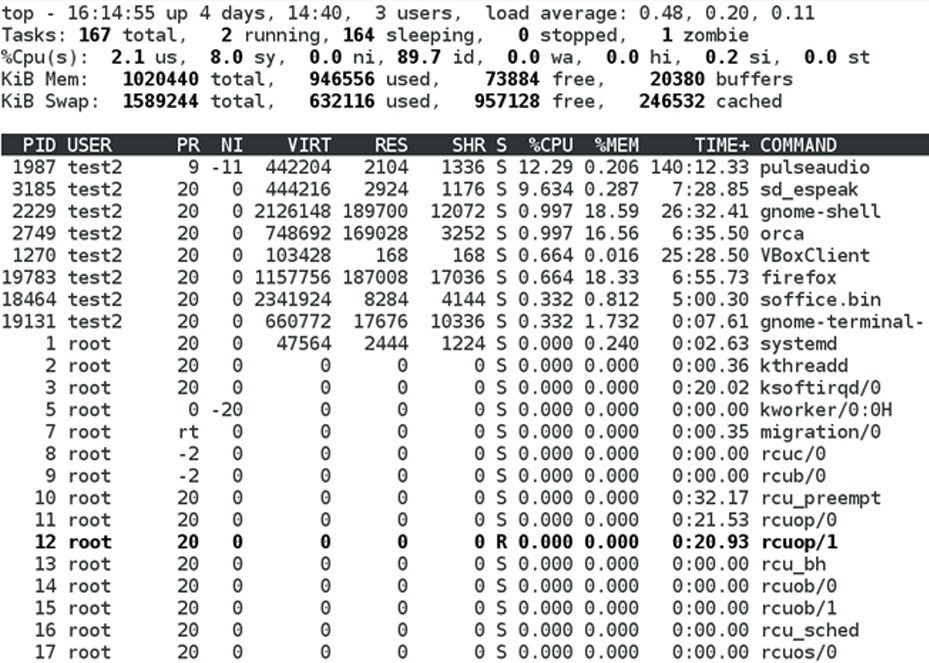
\includegraphics[width=11cm]{c4_top.jpg}
  \end{figure}
\end{frame}

\begin{frame}
  \frametitle{常用命令 | 进程管理 | top}
  The first line of the \textbf{top} output displays a quick summary of what is happening in the system including:
  \begin{itemize}
    \item How long the system has been up
    \item How many users are logged on
    \item What is the load average
  \end{itemize}
  The \textbf{load average} determines how busy the system is. A load average of 1.00 per CPU indicates a fully subscribed, but not overloaded, system. If the load average goes above this value, it indicates that processes are competing for CPU time. If the load average is very high, it might indicate that the system is having a problem, such as a runaway process (a process in a non-responding state).
\end{frame}

\begin{frame}
  \frametitle{常用命令 | 进程管理 | top}
  The second line of the \textbf{top} output displays the total number of processes, the number of running, sleeping, stopped and zombie processes. Comparing the number of running processes with the load average helps determine if the system has reached its capacity or perhaps a particular user is running too many processes. The stopped processes should be examined to see if everything is running correctly.
\end{frame}

\begin{frame}
  \frametitle{常用命令 | 进程管理 | top}
  The third line of the \textbf{top} output indicates how the CPU time is being divided between the users (\textbf{us}) and the kernel (\textbf{sy}) by displaying the percentage of CPU time used for each.\\
  \vspace{0.3cm}
  The percentage of user jobs running at a lower priority (niceness - \textbf{ni}) is then listed. Idle mode (\textbf{id}) should be low if the load average is high, and vice versa. The percentage of jobs waiting (\textbf{wa}) for I/O is listed. Interrupts include the percentage of hardware (\textbf{hi}) vs.  software interrupts (\textbf{si}). Steal time (\textbf{st}) is generally used with virtual machines, which has some of its idle CPU time taken for other uses.
\end{frame}

\begin{frame}
  \frametitle{常用命令 | 进程管理 | top}
  The fourth and fifth lines of the \textbf{top} output indicate memory usage, which is divided in two categories:
  \begin{itemize}
    \item Physical memory (RAM) – displayed on line 4.
    \item Swap space – displayed on line 5.
  \end{itemize}
  Both categories display total memory, used memory, and free space.\\
  \vspace{0.3cm}
  You need to monitor memory usage very carefully to ensure good system performance. Once the physical memory is exhausted, the system starts using \textbf{swap} space (temporary storage space on the hard drive) as an extended memory pool, and since accessing disk is much slower than accessing memory, this will negatively affect system performance.\\
  \vspace{0.3cm}
  If the system starts using swap often, you can add more swap space. However, adding more physical memory should also be considered.
\end{frame}

\begin{frame}
  \frametitle{常用命令 | 进程管理 | top}
  Each line in the process list of the \textbf{top} output displays information about a process. By default, processes are ordered by highest CPU usage. The following information about each process is displayed: 
  \begin{itemize}
    \item Process Identification Number (PID)
    \item Process owner (USER)
    \item Priority (PR) and nice values (NI)
    \item Virtual (VIRT), physical (RES), and shared memory (SHR)
    \item Status (S)
    \item Percentage of CPU (\%CPU) and memory (\%MEM) used
    \item Execution time (TIME+)
    \item Command (COMMAND)
  \end{itemize}
\end{frame}

\begin{frame}
  \frametitle{常用命令 | 进程管理 | top}
  {\footnotesize
  Besides reporting information, \textbf{top} can be utilized interactively for monitoring and controlling processes. While \textbf{top} is running in a terminal window you can enter single-letter commands to change its behaviour. For example, you can view the top-ranked processes based on CPU or memory usage. If needed, you can alter the priorities of running processes or you can stop/kill a process.
  }
  \vspace{-0.2cm}
  \begin{figure}
    \centering
    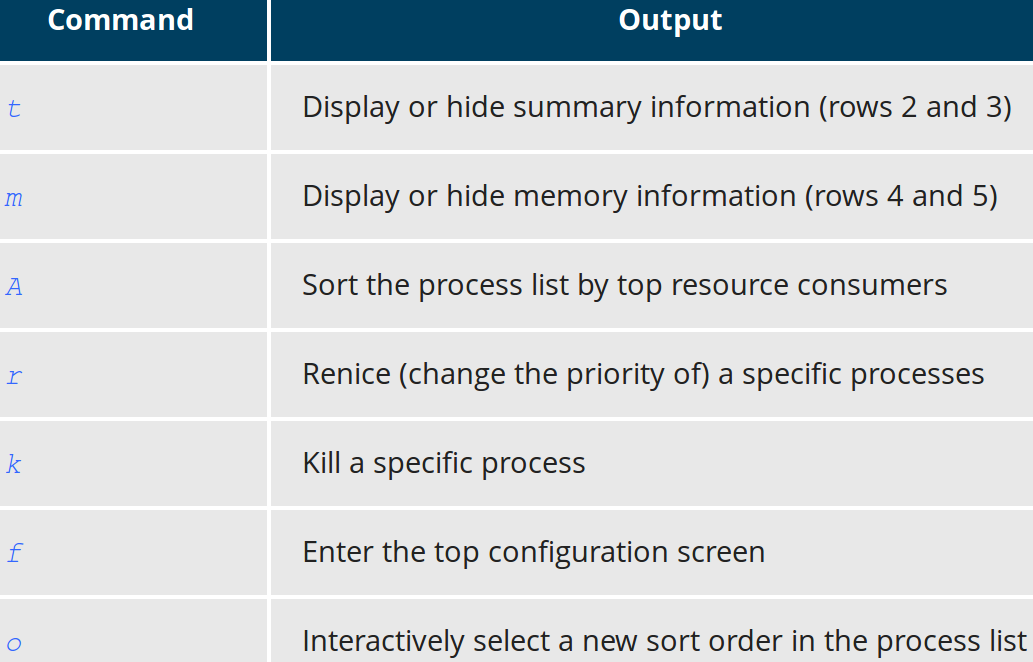
\includegraphics[width=11cm,height=5.3cm]{c4_top_key.png}
  \end{figure}
\end{frame}

\begin{frame}[fragile]
  \frametitle{常用命令 | 进程管理 | top}
  \begin{block}{作用}
    进程状态显示和进程控制;动态显示(每5秒钟自动刷新一次)。
  \end{block}
  \pause
  \begin{block}{选项}
    \begin{itemize}
      \item c:显示整个命令行而不仅仅显示命令名
      \item d:指定刷新的时间间隔
    \end{itemize}
  \end{block}
  \pause
  \begin{block}{命令}
    \begin{itemize}
      \item h,?:获得帮助
      \item k:终止执行中的进程
      \item r:重新设置进程优先级
      \item s:改变刷新的时间间隔
      \item u:查看指定用户的进程
      \item W:将当前设置写入 \verb|~/.toprc| 文件中
    \end{itemize}
  \end{block}
\end{frame}

\begin{frame}
  \frametitle{常用命令 | 进程管理 | ps | 选项}
  \begin{block}{选项}
    \begin{itemize}
      \item a:显示所有用户的进程
      \item e:显示所有进程,包括没有控制终端的进程
      \item l:(小写L)长格式显示
      \item u:显示用户名和启动时间
      \item w:宽行显示,可以使用多个w进行加宽显示
      \item x:显示没有控制终端的进程
    \end{itemize}
  \end{block}
\end{frame}

\begin{frame}
  \frametitle{常用命令 | 进程管理 | ps | 实例}
  \begin{block}{实例}
    \begin{itemize}
      \item ps:查看隶属于自己的进程
      \item ps -u or -l:查看隶属于自己的进程的详细信息
      \item ps -le or -aux:查看所有用户执行的进程的详细信息
      \item ps -aux -\!-sort pid:可按进程执行的时间、PID、UID等对进程进行排序
      \item ps -aux | grep USER,ps -uU USER:查看系统中指定用户执行的进程
      \item ps -le | grep PROCESS:查看指定进程信息
    \end{itemize}
  \end{block}
\end{frame}

\begin{frame}
  \frametitle{常用命令 | 进程管理 | ps | 解读}
  \begin{block}{信息解读}
    \begin{itemize}
      \item PID:进程号
      \item PPID:父进程的进程号
      \item TTY:进程启动的终端
      \item STAT:进程当前状态(S休眠状态,D不可中断的休眠状态,R运行状态,Z僵死状态,T停止)
      \item NI:进程优先级
      \item TIME:进程自从启动以来启用CPU的总时间
      \item COMMAND/CMD:进程的命令名
      \item USER:用户名
      \item \%CPU:占用CPU时间和总时间的百分比
      \item \%MEM:占用内存与系统内存总量的百分比
    \end{itemize}
  \end{block}
\end{frame}

\begin{frame}[fragile]
  \frametitle{常用命令 | 进程管理 | ps | System V Style}
  \textbf{ps} provides information about currently running processes, keyed by \textbf{PID}. If you want a repetitive update of this status, you can use \textbf{top} or commonly installed variants such as \textbf{htop} or \textbf{atop} from the command line, or invoke your distribution's graphical system monitor application.\\
  \vspace{0.2cm}
  \textbf{ps} has many options for specifying exactly which tasks to examine, what information to display about them, and precisely what output format should be used.\\
  \vspace{0.2cm}
  Without options \textbf{ps} will display all processes running under the current shell. You can use the \verb|-u| option to display information of processes for a specified username. The command \verb|ps -ef| displays all the processes in the system in full detail. The command \verb|ps -eLf| goes one step further and displays one line of information for every \textbf{thread} (remember, a process can contain multiple threads).
\end{frame}

\begin{frame}[fragile]
  \frametitle{常用命令 | 进程管理 | ps | BSD Style}
  \textbf{ps} has another style of option specification which stems from the \textbf{BSD} variety of UNIX, where options are specified without preceding dashes.  For example, the command \verb|ps aux| displays all processes of all users. The command \verb|ps axo| allows you to specify which attributes you want to view.
  \begin{figure}
    \centering
    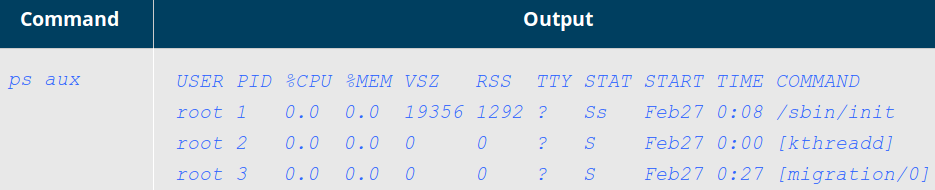
\includegraphics[width=11cm]{c4_ps_aux.png}\\
    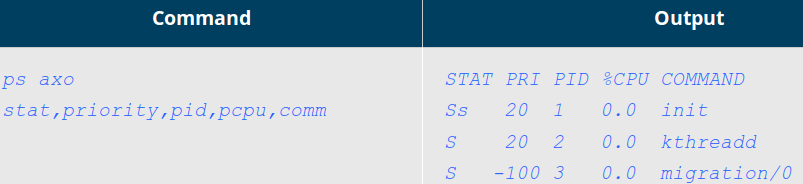
\includegraphics[width=11cm]{c4_ps_axo.png}
  \end{figure}
\end{frame}

\begin{frame}
  \frametitle{常用命令 | 进程管理 | pstree}
  \begin{columns}
    \column{0.4\textwidth}
  \textbf{pstree} displays the processes running on the system in the form of a \textbf{tree diagram} showing the relationship between a process and its parent process and any other processes that it created. Repeated entries of a process are not displayed, and threads are displayed in curly braces.
    \column{0.6\textwidth}
    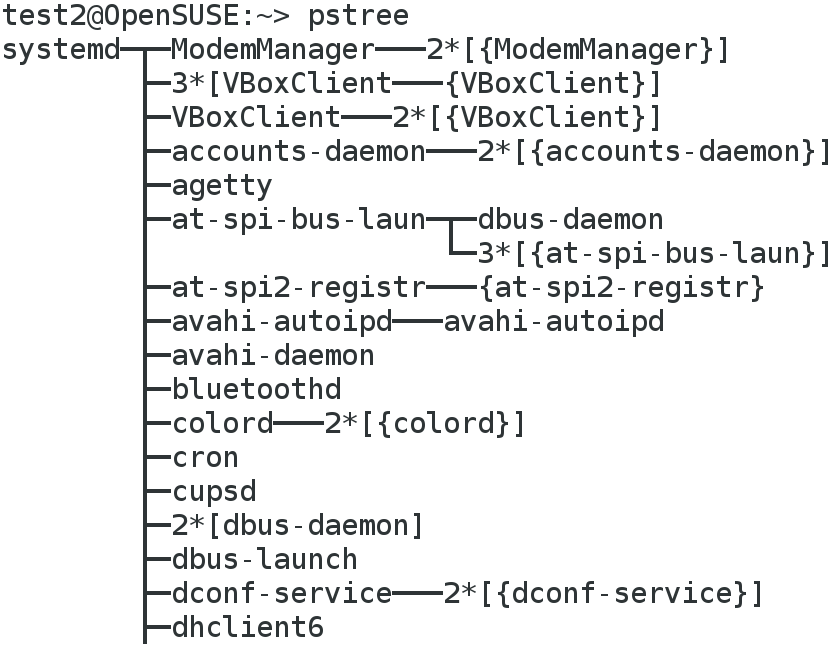
\includegraphics[width=\textwidth]{c4_pstree.jpg}
  \end{columns}
\end{frame}

\begin{frame}[fragile]
  \frametitle{常用命令 | 进程管理 | kill}
  \begin{itemize}
    \item 关闭进程:kill 进程号
    \item 强行关闭:kill -9 进程号
    \item 重启进程:kill -1 进程号
    \item 关闭图形程序:xkill
    \item 结束所有进程:killall
    \item 查找服务进程号:pgrep 服务名称
    \item 关闭进程:pkill 进程名称
  \end{itemize}
  To terminate a process you can type \verb|kill -SIGKILL <pid>| or \verb|kill -9 <pid>|. Note however, you can only \textbf{kill} your own processes: those belonging to another user are off limits unless you are root.
\end{frame}

\begin{frame}[fragile]
  \frametitle{常用命令 | 进程管理 | Background and Foreground}
  {\footnotesize
  Linux supports \textbf{background} and \textbf{foreground} job processing. (A job in this context is just a command launched from a terminal window.) \textbf{Foreground} jobs run directly from the shell, and when one foreground job is running, other jobs need to wait for shell access (at least in that terminal window if using the GUI) until it is completed. This is fine when jobs complete quickly. But this can have an adverse effect if the current job is going to take a long time (even several hours) to complete.\\
  \vspace{0.2cm}
  In such cases, you can run the job in the \textbf{background} and free the shell for other tasks. The background job will be executed at lower priority, which, in turn, will allow smooth execution of the interactive tasks, and you can type other commands in the terminal window while the background job is running. By default all jobs are executed in the foreground. You can put a job in the background by suffixing \verb|&| to the command, for example: \verb|updatedb &|.\\
  \vspace{0.2cm}
  You can either use \textbf{CTRL-Z} to suspend a foreground job or \textbf{CTRL-C} to terminate a foreground job and can always use the \textbf{bg} and \textbf{fg} commands to run a process in the background and foreground, respectively.\\
  } 
\end{frame}

\begin{frame}[fragile]
  \frametitle{常用命令 | 进程管理 | Managing Jobs}
  The \textbf{jobs} utility displays all jobs running in background. The display shows the job ID, state, and command name, as shown here.\\
  \vspace{0.2cm}
  \verb|jobs -l| provides the same information as \verb|jobs| including the PID of the background jobs.\\
  \vspace{0.2cm}
  The background \textbf{jobs} are connected to the terminal window, so if you log off, the jobs utility will not show the ones started from that window.
\end{frame}

\begin{frame}
  \frametitle{常用命令 | 进程管理 | \alert{挂起和恢复}}
  \begin{itemize}
    \item 进程的挂起(中止):Ctrl+Z
    \item 进程的终止:Ctrl+C
    \item 恢复挂起/后台的进程到前台继续运行:fg
    \item 恢复挂起/后台的进程到后台继续运行:bg
    \item 查看后台挂起或正在运行的进程:jobs
  \end{itemize}
\end{frame}

\begin{frame}
  \frametitle{常用命令 | 进程管理 | 挂起和恢复}
  \begin{figure}
    \centering
    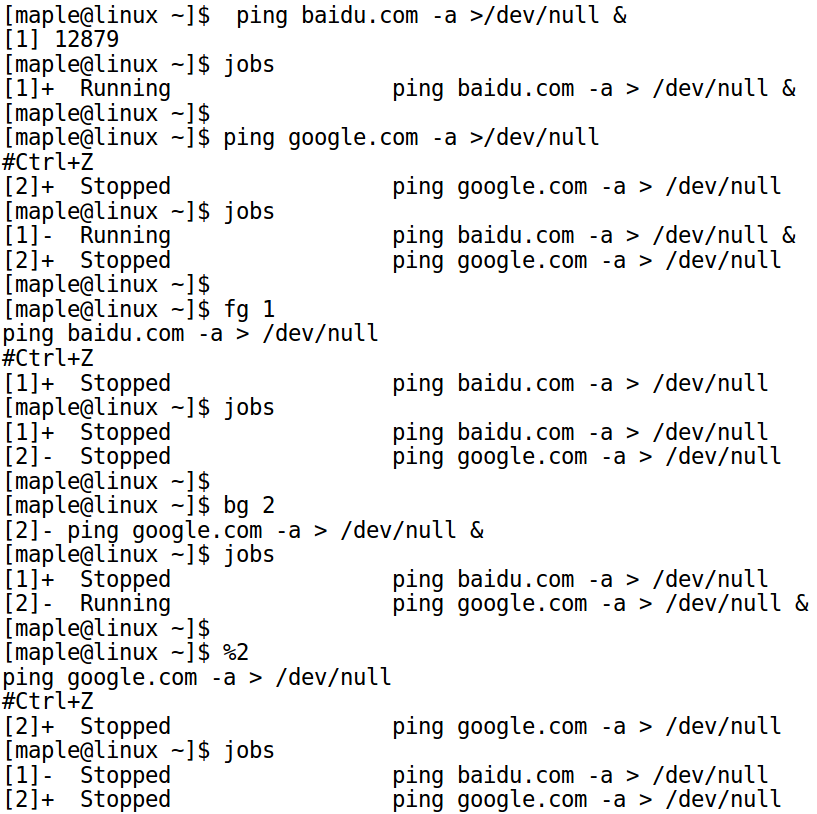
\includegraphics[width=11cm,height=7.5cm]{c4_jobs.png}
  \end{figure}
\end{frame}

\begin{frame}
  \frametitle{常用命令 | 进程管理 | \alert{计划任务}}
  \begin{itemize}
    \item at:安排(非交互式)作业在指定时间执行一次
    \item batch:安排作业在系统负载不重(平均负载降到0.8以下)时执行一次
    \item cron:安排周期性运行的作业
    \item crontab:用于生成cron进程所需要的crontab文件
  \end{itemize}
\end{frame}

\begin{frame}
  \frametitle{常用命令 | 进程管理 | 计划任务 | at}
  Suppose you need to perform a task on a specific day sometime in the future. However, you know you will be away from the machine on that day. How will you perform the task? You can use the \textbf{at} utility program to execute any non-interactive command at a specified time, as illustrated in the diagram.
  \begin{figure}
    \centering
    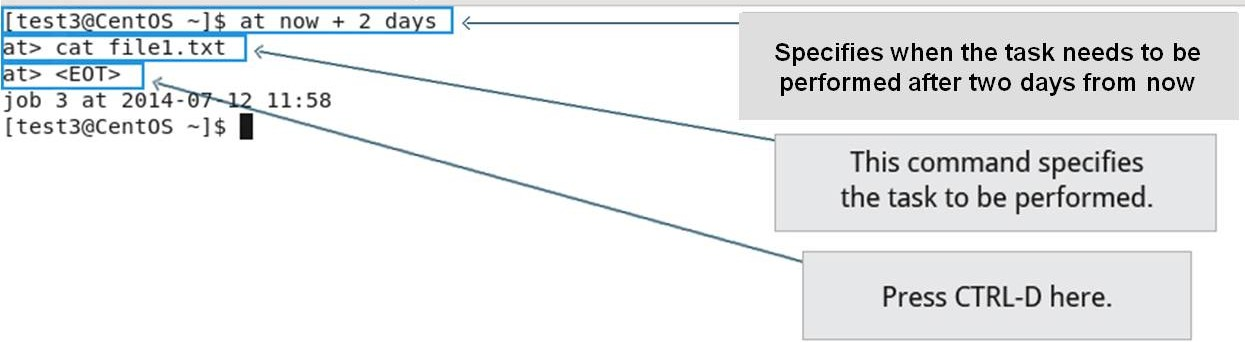
\includegraphics[width=12cm]{c4_at.jpg}
  \end{figure}
\end{frame}

\begin{frame}[fragile]
  \frametitle{常用命令 | 进程管理 | 计划任务 | cron}
  {\footnotesize
  \textbf{cron} is a time-based scheduling utility program. It can launch routine background jobs at specific times and/or days on an on-going basis.  \textbf{cron} is driven by a configuration file called \verb|/etc/crontab| (\textbf{cron} table) which contains the various shell commands that need to be run at the properly scheduled times. There are both system-wide crontab files and individual user-based ones. Each line of a crontab file represents a job, and is composed of a so-called CRON expression, followed by a shell command to execute.\\
  The \verb|crontab -e| command will open the crontab editor to edit existing jobs or to create new jobs. Each line of the crontab file will contain 6 fields.\\
  }
  \vspace{-0.2cm}
  \begin{figure}
    \centering
    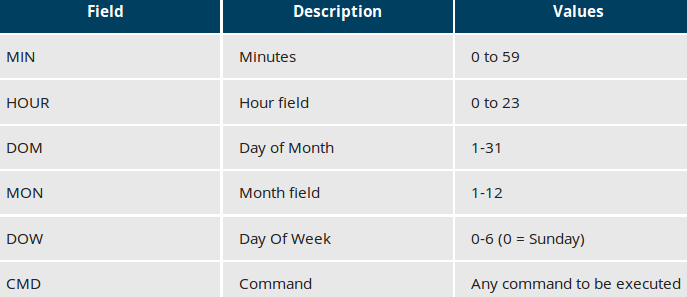
\includegraphics[width=10cm]{c4_cron.png}
  \end{figure}
\end{frame}

\begin{frame}[fragile]
  \frametitle{常用命令 | 进程管理 | 计划任务 | cron | Example}
\begin{lstlisting}
* * * * * /usr/local/bin/execute/this/script.sh
30 08 10 06 * /home/sysadmin/full-backup
\end{lstlisting}
\pause
\begin{enumerate}
  \item Schedule a job to execute `script.sh' every minute of every hour of every day of the month, and every month and every day in the week.
  \item Schedule a full-backup at 8.30am, 10-June irrespective of the day of the week.
\end{enumerate}
\end{frame}

\begin{frame}[fragile]
  \frametitle{常用命令 | 进程管理 | 计划任务 | sleep}
  \textbf{sleep} suspends execution for at least the specified period of time, which can be given as the number of seconds (the default), minutes, hours or days. After that time has passed (or an interrupting signal has been received) execution will resume. Syntax:\\
  \vspace{0.1cm}
  \verb|sleep NUMBER[SUFFIX]...|\\
  \vspace{0.1cm}
  where SUFFIX may be:
  \begin{enumerate}
    \item s for seconds (the default)
    \item m for minutes
    \item h for hours
    \item d for days
  \end{enumerate}
  \textbf{sleep} and \textbf{at} are quite different; \textbf{sleep} delays execution for a specific period while \textbf{at} starts execution at a later time.
\end{frame}

\begin{frame}
  \frametitle{常用命令 | 进程管理 | \alert{nohup}}
  \begin{block}{用途}
    通过让提交的命令忽略HUP(hangup)信号,使进程在用户退出登录后仍旧继续执行。\\ nohup命令将执行后的数据信息和错误信息默认储存到文件nohup.out中。\\ \alert{远程登录服务器运行大型程序时常用/必用!}
  \end{block}
  \pause
  \begin{block}{使用}
    nohup COMMADN/PROGRAM \& \\
    nohup COMMAND/PROGRAM > nohup2.out 2>\&1 \&
  \end{block}
\end{frame}

\subsection{压缩解压}
\begin{frame}
  \frametitle{常用命令 | \alert{压缩解压}}
  \begin{table}
    \centering
    \rowcolors[]{1}{blue!20}{blue!10}
    \begin{tabularx}{\textwidth}{ccXX}
      \hline
      \rowcolor{blue!50}命令 & 助记 & 说明 & 常用后缀\\
      \hline
      tar & Tape ARchive & 创建磁盘归档(打包/归档) & .tar\\
      gzip & GNU Zip & 压缩 & .gz, .z, .Z, (.tar.gz, .tgz)\\
      gunzip & --- & 解压 & .gz, .z, .Z, (.tar.gz, .tgz)\\
      bzip2 & --- & 压缩 & .bz, .bz2, .bzip2, (.tar.bz, .tbz, .tbz2)\\
      bunzip2 & --- & 解压 & .bz, .bz2, .bzip2, (.tar.bz, .tbz, .tbz2)\\
      xz & --- & 压缩 & .xz\\
      unxz & --- & 解压 & .xz\\
      zip & --- & 压缩 & .zip\\
      unzip & --- & 解压 & .zip\\
      \hline
    \end{tabularx}
  \end{table}
\end{frame}

\begin{frame}
  \frametitle{常用命令 | \alert{压缩解压}}
  \begin{table}
    \centering
    \rowcolors[]{1}{blue!20}{blue!10}
    \begin{tabularx}{\textwidth}{cX}
      \hline
      \rowcolor{blue!50}命令 & 说明\\
      \hline
      gzip & Linux中使用最广泛\\
      bzip2 & 压缩后的文件比gzip节省空间(压缩时间长)\\
      xz & 压缩后的文件在Linux中是最节省空间的(压缩时间更长)\\
      zip & 和其他操作系统(如Windows)的兼容性好\\
      \hline
    \end{tabularx}
  \end{table}
  备注:归档是否是压缩的和采用哪种压缩方式并不取决于其扩展名,扩展名只是为了便于辨识。
\end{frame}

\begin{frame}
  \frametitle{常用命令 | 压缩解压 | \alert{tar}}
  \begin{table}
    \centering
    \rowcolors[]{1}{blue!20}{blue!10}
    \begin{tabularx}{0.9\textwidth}{ccX}
      \hline
      \rowcolor{blue!50}选项 & 助记 & 说明\\
      \hline
      -c & Create & 创建文件(打包)\\
      -f & File & 指定打包文件或设备\\
      -j & --- & 使用bzip2压缩/解压\\
      -r & append & 向包中(末尾)追加文件\\
      -t & lisT & 显示包中的内容\\
      -u & Update & 更新包中的内容或添加新内容\\
      -v & Verbose & 显示详细的打包过程\\
      -x & eXtract & 提取文件(解包)\\
      -z & gZip & 使用gzip压缩/解压\\
      \hline
    \end{tabularx}
  \end{table}
\end{frame}

\begin{frame}[fragile]
  \frametitle{常用命令 | 压缩解压 | \alert{tar}}
  \begin{block}{常用命令}
    \begin{itemize}
      \item tar归档、gzip压缩 /etc目录:\\ \verb|tar -cvzf /backups/etc_backup.tar.gz /etc|
      \item gzip解压缩、tar解归档:\\ \verb|tar -xvzf /backups/etc_backup.tgz|
      \item tar归档、bzip2压缩 /etc目录:\\ \verb|tar -cvjf /backups/etc_backup.tar.bz /etc|
      \item bzip2解压缩、tar解归档:\\ \verb|tar -xvjf /backups/etc_backup.tbz|
    \end{itemize}
  \end{block}
\end{frame}

\subsection{网络通信}
\begin{frame}
  \frametitle{常用命令 | 网络通信}
  \begin{table}
    \centering
    \rowcolors[]{1}{blue!20}{blue!10}
    \begin{tabularx}{0.8\textwidth}{cX}
      \hline
      \rowcolor{blue!50}命令 & 说明\\
      \hline
      write & 向另外一个用户发送信息,以Ctrl+D结束\\
      wall & 向所有用户广播信息\\
      ping & 测试网络连通性\\
      hostname & 查看本机的hostname\\
      ifconfig & 查看网络设置信息\\
      route & 显示和操作IP路由表\\
      ip & 整合了ifconfig和route两个命令\\
      \hline
    \end{tabularx}
  \end{table}
\end{frame}

\begin{frame}
  \frametitle{常用命令 | 网络通信}
  \begin{table}
    \centering
    \rowcolors[]{1}{blue!20}{blue!10}
    \begin{tabularx}{0.8\textwidth}{cX}
      \hline
      \rowcolor{blue!50}命令 & 说明\\
      \hline
      traceroute & 追踪数据包在网络上传输时的全部路径\\
      host & 返回一个主机的网络地址或返回主机名\\
      nslookup & 查询一台机器的IP地址和其对应的域名\\
      dig & 域名查询工具\\
      ethtool & 查询及设置网卡参数\\
      netstat & 显示各种网络相关信息\\
      nmap & 网络扫描和嗅探工具包\\
      tcpdump & 网络数据采集分析工具\\
      iptraf & 实时地监视网卡流量\\
      \hline
    \end{tabularx}
  \end{table}
\end{frame}

\begin{frame}[fragile]
  \frametitle{常用命令 | 网络通信}
  \begin{table}
    \centering
    \rowcolors[]{1}{blue!20}{blue!10}
    \begin{tabularx}{0.9\textwidth}{cX}
      \hline
      \rowcolor{blue!50}命令 & 说明\\
      \hline
      ssh & 远程登录客户端工具\\
      scp & \footnotesize{基于SSH登录进行安全的远程文件拷贝(Secure CoPy)}\\
      wget & 命令行下载工具\\
      curl & 利用URL规则在命令行下工作的文件传输工具\\
      http & httpie: CLI, cURL-like tool for humans\\
      \hline
      ftp, sftp & 命令行下的FTP客户端\\
      ncftp, yafc & 命令行下的FTP客户端,支持Windows和Linux\\
      lftp & 功能强大的文件传输客户端程序,支持FTP、SSH和HTTP等多种文件传输协议\\
      \hline
      lynx & 字符界面下的全功能的WWW浏览器\\
      links, elinks & 基于lynx,支持frame、表格和鼠标\\
      w3m & 较新的命令行下的网页浏览器\\
      \hline
    \end{tabularx}
  \end{table}
\end{frame}

\subsection{关机重启}
\begin{frame}
  \frametitle{常用命令 | \alert{关机重启}}
  \begin{table}
    \centering
    \rowcolors[]{1}{blue!20}{blue!10}
    \begin{tabularx}{0.9\textwidth}{cX}
      \hline
      \rowcolor{blue!50}命令 & 说明\\
      \hline
      shutdown & 关闭系统\\
      reboot & 重新启动系统\\
      halt & 立即关闭系统\\
      poweroff & 通过切断电源来关闭系统\\
      \hline
    \end{tabularx}
  \end{table}
\end{frame}

\subsection{获取帮助}
\begin{frame}[fragile]
  \frametitle{常用命令 | \alert{获取帮助}}
  \begin{table}
    \centering
    \rowcolors[]{1}{blue!20}{blue!10}
    \begin{tabularx}{0.9\textwidth}{ccX}
      \hline
      \rowcolor{blue!50}命令 & 助记 & 说明\\
      \hline
      man & MANual & 查看命令的联机帮助页\\
      info & Info format & 查看命令的信息帮助页\\
      apropos & --- & 使用关键字来查找文件\\
      whatis & --- & 显示联机帮助页中对命令的简短描述\\
      makewhatis & --- & 建立 whatis 和 apropos 搜索使用的数据库\\
      whereis & --- & 查找软件包\\
      -\!-help/-h & --- & 命令的 -\!-help/-h选项\\
      \hline
    \end{tabularx}
  \end{table}
\end{frame}


\section{命令使用技巧}
\subsection{补全、历史和别名}
\begin{frame}[fragile]
  \frametitle{命令技巧 | 补全、历史和别名}
  \begin{block}{自动补全}
    自动补全/补齐允许用户输入命令或文件名起始的若干个字母后,按$\Tab$(\alert{Tab})补全命令名或文件名。
  \end{block}
  \pause
  \begin{block}{命令历史}
    %命令历史允许用户浏览先前输入的命令并重新调用它们,用history命令可以显示命令列表,按方向键$\UArrow$和$\DArrow$可查找以前执行过的命令。
    命令历史允许用户浏览先前输入的命令并重新调用它们,用 \alert{history} 命令可以显示命令列表,按方向键(上、下)可查找以前执行过的命令。
  \end{block}
  \pause
  \begin{block}{命令别名}
    \begin{itemize}
      \item \alert{alias} 查看、定义别名;unalias删除别名
      \item \verb|alias ll="ls -l"|; \quad \verb|alias la="ls -al"|; \verb|alias cd3="cd ../../.."|
      \item \verb|alias ls="ls -l"|; 执行原始的ls命令:\verb|\ls|
    \end{itemize}
  \end{block}
\end{frame}

\subsection{命令连接符和后台运行}
\begin{frame}[fragile]
  \frametitle{命令技巧 | \alert{连接符}}
  \begin{block}{命令连接符}
    \begin{description}
      \item[;] 用 \verb|;| 间隔的各命令按顺序依次执行
      \item[\&\&] 前后命令的执行存在逻辑与关系:只有 \verb|&&| 前面的命令执行成功后,它后面的命令才被执行
      \item[||] 前后命令的执行存在逻辑或关系:只有 \verb=||= 前面的命令执行失败后,它后面的命令才被执行。
    \end{description}
  \end{block}
  \pause
  \vspace{-0.5em}
  \begin{block}{后台运行}
    \begin{itemize}
      \item \verb|COMMAND &|:后台运行,关掉客户端/终端会停止运行
      \item \verb|nohup COMMAND &|:后台运行,关掉客户端/终端仍会继续运行
    \end{itemize}
  \end{block}
  \pause
  \vspace{-0.5em}
  \begin{block}{在子shell中运行命令:(CMD)}
    \begin{itemize}
      \item 在其它目录运行一个命令,然后自动返回当前工作目录
      \item \verb|(cd /tmp; ls)|
    \end{itemize}
  \end{block}
\end{frame}

\begin{frame}
  \frametitle{命令技巧 | 连接符 | 实例}
  \begin{figure}
  \centering
    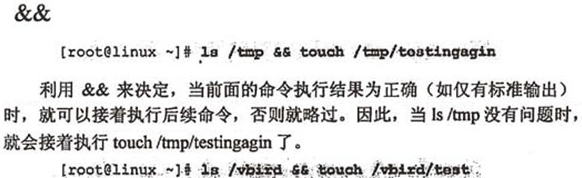
\includegraphics[width=11cm]{c4_andor_01.jpg}
    \vspace{0.3cm}
    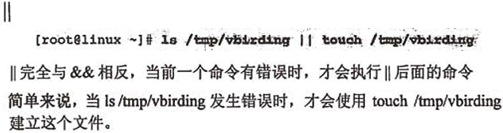
\includegraphics[width=11cm]{c4_andor_02.png}
  \end{figure}
\end{frame}

\begin{frame}[fragile]
  \frametitle{命令技巧 | 连接符 | 实例}
  \begin{description}
     \item[mkdir test; cd test] 创建文件夹,并成功切换进去
     \item[cd test; mkdir test] 切换文件夹报错,创建文件夹
     \item[mkdir test \&\& cd test] 创建文件夹,并成功切换进去
     \item[cd test \&\& mkdir test] 切换文件夹报错,不会创建文件夹
     \item[mkdir test || cd test] 创建文件夹,但不会切换进去
     \item[cd test || mkdir test] 切换文件夹报错,但会创建文件夹
  \end{description}
\end{frame}

\subsection{终端快捷键}
\begin{frame}
  \frametitle{命令技巧 | 快捷键}
  \begin{table}
    \centering
    \rowcolors[]{1}{blue!20}{blue!10}
    \begin{tabularx}{0.4\textwidth}{cX}
      \hline
      \rowcolor{blue!50}快捷键 & 作用\\
      \hline
      clear & 清屏\\
      \alert{Ctrl+L} & 清屏\\
      \hline
      Ctrl+S & 阻止屏幕输出\\
      Ctrl+Q & 恢复屏幕输出\\
      \hline
      \alert{Ctrl+C} & 终止命令\\
      \alert{Ctrl+Z} & 挂起命令\\
      \hline
      \alert{Ctrl+D} & 注销会话\\
      exit & 注销会话\\
      \hline
    \end{tabularx}
  \end{table}
\end{frame}

\begin{frame}
  \frametitle{命令技巧 | 快捷键(续)}
  \begin{table}
    \centering
    \rowcolors[]{1}{blue!20}{blue!10}
    \begin{tabularx}{0.6\textwidth}{cX}
      \hline
      \rowcolor{blue!50}快捷键 & 作用\\
      \hline
      Ctrl+A & 移动到命令行首\\
      Ctrl+E & 移动到命令行尾\\
      Ctrl+F & 按字符前/右移\\
      Ctrl+B & 按字符后/左移\\
      \hline
      Ctrl+U & 从光标处删除至命令行首\\
      Ctrl+K & 从光标处删除至命令行尾\\
      Ctrl+W & 从光标处删除至字首\\
      Ctrl+H & 删除光标前的字符\\
      Ctrl+D & 删除光标处的字符\\
      Ctrl+T & 交换光标前的两个字符\\
      Ctrl+Y & 粘贴上次的删除\\
      Ctrl+\_ & 撤销操作\\
      \hline
    \end{tabularx}
  \end{table}
\end{frame}

\begin{frame}[fragile]
  \frametitle{命令技巧 | 快捷键(续)}
  \begin{table}
    \centering
    \rowcolors[]{1}{blue!20}{blue!10}
    \begin{tabularx}{0.8\textwidth}{cX}
      \hline
      \rowcolor{blue!50}快捷键 & 作用\\
      \hline
      \alert{Ctrl+R} & 逆向搜索命令历史\\
      Ctrl+G & 退出历史搜索模式\\
      \hline
      Ctrl+P & 历史中的上一条命令\\
      Ctrl+N & 历史中的下一条命令\\
      \hline
      \alert{!!} & 执行上一条命令\\
      !ABC & 执行最近的以ABC开头的命令\\
      !ABC:p & 仅打印输出而不执行\\
      \hline
      \verb|!^| & 上一条命令的第一个参数\\
      \verb|!^:p| & 打印输出上一条命令的第一个参数\\
      \verb|!$| & 上一条命令的最后一个参数\\
      \verb|!$:p| & 打印输出上一条命令的最后一个参数\\
      \verb|!*| & 上一条命令的所有参数\\
      \verb|!*:p| & 打印输出上一条命令的所有参数\\
      \hline
      \verb|^A^B| & 将上一条命令中的第一个A替换为B并执行\\
      \verb|^A^B^| & 将上一条命令中的所有A替换为B并执行\\
      \hline
    \end{tabularx}
  \end{table}
\end{frame}

\section{回顾与总结}
\subsection{总结}
\begin{frame}[fragile]
  \frametitle{Linux命令 | 总结}
  \begin{block}{知识点}
    \begin{itemize}
      \item Linux命令的基本结构:命令、参数(选项、目标)
      \item 查找命令相关信息的方法:man、info、-\!-help/-h、apropos
      \item 命令的修改:通配符、转义符、输入输出重定向、管道、命令置换
      \item 目录和文件操作、权限管理、系统导航、压缩解压等常用命令
      \item 命令使用技巧:补全、历史、别名、连接符、后台运行、快捷键
    \end{itemize}
  \end{block}
  \begin{block}{技能}
    \begin{itemize}
      \item 常用命令及其选项的使用
      \item 命令的修改
      \item 命令的使用技巧
    \end{itemize}
  \end{block}
\end{frame}

\subsection{思考题}
\begin{frame}
  \frametitle{Linux命令 | 思考题}
  \begin{enumerate}
    \item Linux命令由哪几部分构成?
    \item 查找命令相关信息的方法有哪些?
    \item 列举三个常用的通配符并举例说明。
    \item 如何进行输入、结果输出和错误输出的重定向?
    \item 命令置换的方法有哪些,举例说明。
    \item 列举几个常用的命令及其常用选项。
    \item 列举命令使用技巧并进行说明。
  \end{enumerate}
\end{frame}

\begin{frame}
  \frametitle{下节预告}
  你是如何处理文本数据(如生物信息学数据)的,包括查找、替换、修改、简单的统计等。\\
  如果是使用Word或Excel来处理的,你有没有想吐槽的地方?
\end{frame}



\section*{Acknowledgements}
\begin{frame}
  \frametitle{Powered by}
  \begin{center}
    
\includegraphics[width=9cm]{power.png}
  \end{center}
\end{frame}

\end{document}


